\documentclass[preview,12pt]{article}
\usepackage{amsmath}
\usepackage{gensymb}
\usepackage{ragged2e}
\usepackage{geometry}
\usepackage{graphicx}
\usepackage{caption}
\usepackage{subcaption}
\usepackage{pdfpages}

\geometry{letterpaper, margin=1in}

\begin{document}

\noindent Compressible Flow and Thermodynamics\newline
Josh Coffey \newline
Assignment 1 \newline
9/3/2020 \newline

\section*{1.1}
    Consider the frictionless, steady flow of a compressible fluid in an infinitesimal stream tube.
    \subsection*{(a)} 
    Demonstrate by the continuity and momentum theorems that
    $$\frac{d\rho}{\rho}+\frac{dA}{A}+\frac{dv}{v}=0$$
    $$dp+\rho v dv+\rho g dz=0$$
    continuity theorem:
    $$\int\int\int\frac{d\rho}{dt}dV+\int\int \rho v_ndA=0$$
    
    know that for steady flow with uniform conditions along control surface, 
    $$\int\int\rho v_ndA=\rho_2v_2A_2-\rho_1v_1A_1=0$$
    Let the left line be "1" and the right line be "2".  Then
    $$\rho_1=\rho$$
    $$v_1=v$$
    $$A_1=A$$
    $$\rho_2=\rho+d\rho$$
    $$A_2=A+dA$$
    $$v_2=v+dv$$
    And the continuity theorem becomes:
    $$\rho A v=(\rho+d\rho)(A+dA)(v+dv)$$
    expanding the right side of the equation gives:
    $$(\rho A + \rho dA+d\rho A+d\rho dA)(v+dv)$$
    $$(\rho Av+\rho dA v+d\rho A v+d\rho dA v+\rho A dv+\rho dA dv+d\rho A dv+d\rho dAdv)$$
    dividing both sides by $\rho Av$
    $$1=1+\frac{dA}{A}+\frac{d\rho}{\rho}+\frac{d\rho dA}{\rho A}+\frac{dv}{v}+\frac{dAdv}{Av}+\frac{d\rho dv}{\rho v}+\frac{d\rho dAdv}{\rho A v}$$
    $$0=\frac{dA}{A}+\frac{d\rho}{\rho}+\frac{dv}{v}+\frac{d\rho dA}{\rho A}+\frac{dAdv}{Av}+\frac{d\rho dv}{\rho v}+\frac{d\rho dAdv}{\rho A v}$$
    Ignoring higher terms and assuming that at the center of a control volume the values opposing values of $\rho, A,$ and $v$ cancel:
    $$0=\frac{dA}{A}+\frac{d\rho}{\rho}+\frac{dv}{v}$$
    
    \noindent momentum equation:
    $$\int\int\int\frac{\partial \rho \vec{v}}{\partial t}dV+\int\int\rho\vec{v}v_ndA=F$$
    because steady flow, $\frac{d\rho}{dt}=0$
    $$\Sigma F=\int\int\rho(\vec{v} \cdot d\vec{A})\vec{v}=\int\int\rho\vec{v}v_ndA$$
    Note that in both edges of the control surface, the velocity is normal to the surface, meaning that $\vec{v}=v_n$.
    $$\Sigma F=\int\int\rho v_n^2dA$$
    can see that there are three forces on the fluid: gravity and the two forces on both ends of the control surface. 
    $$F_1=\int\int\rho v_n^2dA$$
    $$F_2=\int\int(\rho+d\rho)(v+dv)^2(dA)$$
    integrating gives
    $$F_1=\rho v^2 A$$
    $$F_2=(\rho+d\rho)(v+dv)^2(A+dA)$$
    $$F_2=(\rho+d\rho)(v^2+2vdv+dv^2)(A+dA)$$
    $$F_2=(\rho v^2 +2\rho vdv+\rho dv^2+d\rho v^2+d\rho 2 vdv+d\rho dv^2)(A+dA)$$
    $$F_2=A\rho v^2 +2A\rho vdv+\rho Adv^2+d\rho v^2+Ad\rho 2 vdv+Ad\rho dv^2+dA\rho v^2 $$
    $$+2dA\rho vdv+dA\rho dv^2+dAd\rho v^2+dAd\rho 2 vdv+dAd\rho dv^2$$
    Again, ignoring higher terms and assuming that opposing values cancel:
    $$F_2=A\rho v^2+2A\rho vdv+Av^2d\rho +\rho v^2dA$$
    Also know that $F_1$ is in the opposite direction of $F_2$
    $$F_1=-\rho v^2 A$$
    Next, assume only gravity and pressure are the only other forces acting on the fluid.  
    $$F_g=-\rho g h=\rho g z$$
    To account for the change in density across the control volume,
    $$F_g=-\frac{1}{2}(\rho+\rho+d\rho) g dz=\frac{d\rho}{2}gdz+\rho gdz$$
    Ignoring higher terms:
    $$F_g=-\rho g dz$$
    $$F_p=p_1A_1-p_2A_2=pA-(p+dp)(A+dA)=pA-(pA+pdA+dpA+dpdA)$$
    $$=pA-pA+2pdA+dpdA=2pdA$$
    At this point I'm not sure what I did wrong, but you would recombine the four forces to get 
    $$dp+\rho v dv+\rho g dz=0$$
    
    
    
    \subsection*{(b)} 
    Determine the integrated forms of these equations for an in-compressible fluid.
    \begin{figure}
        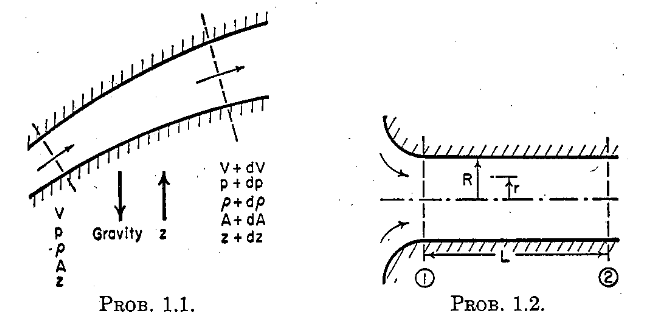
\includegraphics[width=\textwidth]{HW1_1and2.PNG}
        \centering
    \end{figure}
    \newline
    integrating the first equation from point 1 to point 2 gives:
    $$ln(\rho_2)-ln(\rho_1)+ln(A_2)-ln(A_1)+ln(v_2)-ln(v_1)=0$$
    integrating the second equation gives:
    $$p_2-p_1+\frac{1}{2}\rho(v_2^2-v_1^2)+\rho g(z_2-z_1)=0$$
    
\section*{1.2}
    An incompressible fluid flows in a pipe of radius $R$.  At the inlet, section 1, the velocity is uniform over the cross section, with a value $V_1$.  At section 2, where the flow is laminar and fully developed, the velocity varies with radius according to the relation
    $$V=V_{max}\left(1-\frac{r^2}{R^2}\right)$$
    \subsection*{(a)} 
        Demonstrate that $\frac{V}{V_{max}}=\frac{1}{2}$. \newline
        Create a control volume between station 1 and 2.  For an incompressible fluid, the conservation of mass says:
        $$0=\int_{c.s.}\rho(\vec{v}\cdot d\vec{A})=-\rho v_1 A_1+\rho v_2 A_2$$
        $$0=-v_1A_1+(v_{max}\left(1-\frac{r^2}{R^2}\right))A_2=-v_1A_1+A_2v_{max}-A_2v_{max}\frac{r^2}{R^2}$$
        $$\frac{v_1A_1}{v_{max}}=A_2-A_2\frac{r^2}{R^2}$$
        $$\frac{v_1}{v_{max}}=\frac{A_2-A_2\frac{r^2}{R^2}}{A_1}$$
        Know that $A_2=\pi R^2$
        $$\frac{v_1}{v_{max}}=\frac{\pi (R^2-r^2)}{A_1}$$
        let $A_1=\pi r'^2$:
        $$\frac{v_1}{v_{max}}=\frac{ (R^2-r^2)}{r'^2}$$
        Assuming the image above is to scale, at station one $r'=R$
        $$\frac{v_1}{v_{max}}=\frac{ (R^2-r^2)}{R^2}=1-\frac{r^2}{R^2}$$
        
    \subsection*{(b)} 
        if $\vec{\tau_w}$ is the average wall shearing stress retarding the flow between sections 1 and 2, find the pressure drop $(p_1-p_2)$ in terms of $V_{max}, \rho, L, r, \textrm{ and } \vec{\tau_w}$.
        
        $$(p_1-p_2)+\frac{1}{2}\rho(v_1^2-v_2^2)=0$$
        $$(p_1-p_2)=\frac{1}{2}\rho(v_1^2-v_2^2)$$
        $$(p_1-p_2)=\frac{1}{2}\rho(v_1^2-v_{max}\left(1-\frac{r^2}{R^2}\right)^2)$$
        Adding a term for a pressure change due to shear stress:
        $$(p_1-p_2)=\frac{1}{2}\rho(v_1^2-v_{max}\left(1-\frac{r^2}{R^2}\right)^2)-\frac{\tau_w}{A_3}$$
        $A_3$ will be the area impacted by the shear stress, i.e. the area next to the walls.
        $$(p_1-p_2)=\frac{1}{2}\rho(v_1^2-v_{max}\left(1-\frac{r^2}{R^2}\right)^2)-\frac{\tau_w}{2\pi(R-r)L}$$        
        

\section*{1.3} 
    The sketch shows a jet pump (ejector or injector) in which a primary stream of high velocity liquid at section 1 entrains a secondary stream of the same liquid at low velocity at section 2.  At the end of the constant-diameter mixing-tube, i.e., at section 3, the streams are thoroughly mixed and uniform in velocity, as the result of friction between the streams. \newline For the purpose of this analysis, assume that at sections 1 and 2 both streams have the same static pressure and that shearing stresses at the walls of the mixing tube are negligible.
    $$\textrm{Assuming that } A_1=0.1ft^2, A_3=1ft^2, V_1=100ft/sec, V_2=10 ft/sec, \textrm{ and } \rho=64.4 lbm/ft^3$$
    \subsection*{(a)} 
        Calculate $V_3$ (ft/sec) \newline
        Begin by assuming steady flow, incompressible fluids, and constant properties.  Then the continuity equation takes the form:
        $$\int\int\rho \vec{v}\cdot\hat{n}ds=0$$
        splitting this into three parts, 1, 2, and 3, and carrying out the integrations gives that:
        $$-\rho A_1v_1-\rho A_2v_2+\rho A_3v_3=0$$
        solving for $v_3$ gives that:
        $$v_3=\frac{v_1A_1+v_2A_2}{A_3}$$
        Have values for $A_1,A_3,v_1,v_2$, just need $A_2$.  Assuming that $A_3=A_1+A_2$, $v_3$ becomes
        $$v_3=\frac{v_1A_1+v_2(A_3-A_1)}{A_3}$$
        $$v_3=19\frac{ft}{s}$$
    \subsection*{(b)} 
        Calculate $p_3-p_1$ (lbf/in$^2$) \newline
        Using Bernoulli's equation between point 1 and point 3 gives:
        $$p_3+\frac{1}{2}\rho v_3^2=p_1+\frac{1}{2}\rho v_1^2$$
        $$p_3-p_1=\frac{1}{2}\rho v_1^2-\frac{1}{2}\rho v_3^2=\frac{1}{2}\rho(v_1^2-v_3^2)$$
        Calculating and including factors to correct units gives
        $$p_3-p_1=310375.8\frac{lbm}{ft*s^2}\frac{1}{32.174}\frac{1}{144}=66.99159\frac{lbf}{in^2}$$ 
    \begin{figure}
        \centering
        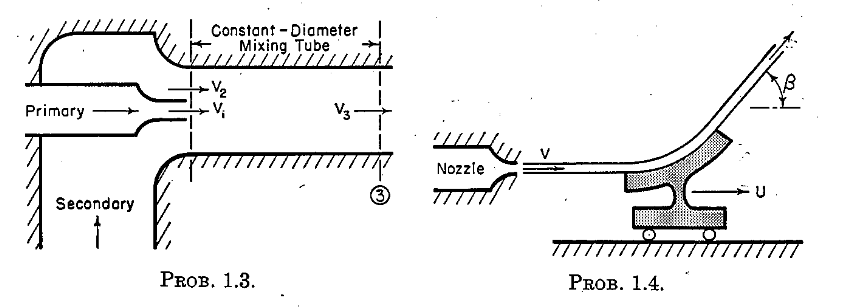
\includegraphics[width=\textwidth]{HW1_3and4.PNG}
    \end{figure}
    
\section*{1.4}
    The sketch shows a vane with a turning angle $\beta$ which moves with steady speed $U$.  The vane receives a jet which leaves a fixed nozzle with speed $V$.
    \subsection*{(a)} 
        Assuming that the vane is mounted on rails as shown in the sketch, show that the work done against the restraining force is a maximum when $U/V=\frac{1}{8}$.
        
        $$W=F\cdot dl$$
        $$\Sigma F=\frac{\partial}{\partial t}\int_{C.V.}\rho \vec{v}dV+\int_{C.S.}\rho(\vec{v}\cdot d\vec{A})\vec{v}$$
        
        
    
    \subsection*{(b)} 
        Assuming that there are a large number of such vanes attached to a rotating wheel moving with peripheral speed $U$, show that the work delivered to the wheel is a maximum when $U/V=\frac{1}{2}$.

\section*{1.5}
    In an experiment to determine drag, a circular cylinder of diameter $d$ was immersed in a steady, two-dimensional, incompressible flow.  Measurements of velocity and pressure were made at the boundaries of the control surface shown.  The pressure was found to be uniform over the entire control surface.  \textit{The x-component of velocity} at the control surface boundary was approximately as indicated by the sketch.  From the measured data, calculate the drag coefficient of the cylinder, based on the projected area and on the free stream dynamic head, $\frac{1}{2}\rho V_0^2$.
    $$C_D=\frac{\textrm{Drag Force per Unit Length}}{\frac{1}{2}\rho v_0^2d}$$
    \begin{figure}
        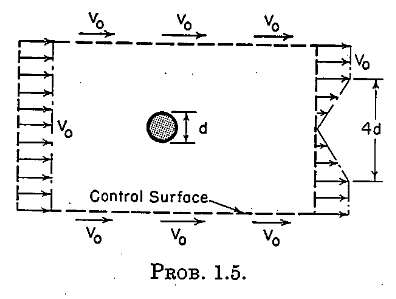
\includegraphics[width=0.5\textwidth]{HW1_5.PNG}
        \centering
    \end{figure}
    $$$$
    Assuming that the center of the cylinder is y=0, the velocity profile takes the form: 
    $$v=v_0-v_0(1-\frac{|y|}{2d}) \textrm{ if }|y|\leq2d$$
    $$v=v_0 \textrm{ if     } |y|\geq2d$$
    Using conservation of mass for an incompressible fluid, and accounting for the top and bottom of the velocity profile, 
    $$\int\int\rho (\vec{v}\cdot\hat{n})dA=0$$
    Assuming $v_3$ and $v_4$ have the same magnitude:
    $$-\rho v_0 A_1+\rho \int_2 v(y)dA+2\dot{m}_{3/4}=0$$
    $$\dot{m}=\frac{1}{2}\rho v_0 A_1-\int_{-2d}^{2d}\frac{\rho}{2}vdy$$
    splitting the integral into two parts to account for the case where y=0:
    $$\dot{m}=\frac{1}{2}\rho v_0 A_1-\frac{\rho}{2}\int_{-2d}^{2d}(v_0-v_0(1-\frac{|y|}{2d}))dy=$$
    $$\dot{m}=\frac{1}{2}\rho v_0 A_1+\frac{\rho}{2d}v_0\int_{0}^{2d}ydy=\frac{1}{2}\rho v_0 A_1+\frac{\rho}{2}v_0d$$
    So we have that:
    $$-\rho v_0 A_1+\rho\int_2v(y)dA+\rho v_0(A_1+d)$$ 
    Assuming all the drag force is in the x-direction:
    $$\Sigma F_x=\int\rho(\vec{v}\cdot d\vec{A})\vec{v}=-\rho v_0^2A_1+\rho\int_2v(y)^2dA+\rho v_0^2(A_1+d)$$
    $$\Sigma F_x=-\rho v_0^2A_1+2\rho\int_0^{2d}\frac{y^2v_0^2}{4d^2}dA+\rho v_0^2(A+d)=-\rho v_0^2A_1+2\rho v_0^2+\rho v_0^2(A_1+d)$$
    Reversing all the signs to make this the drag force:
    $$F_d=\rho v_0^2(A_1-2-A_1-d)=-\rho v_0^2(2-d)$$
    Putting this in the equation for the drag coefficient:
    $$C_d=\frac{-\rho v_0^2(2-d)}{\frac{1}{2}\rho v_0^2d}=\frac{-4-2d}{d}=-\frac{4}{d}-2$$
\end{document}
